\documentclass[sigconf, nonacm]{acmart}

\AtBeginDocument{%
  \providecommand\BibTeX{{%
    Bib\TeX}}}

\settopmatter{printacmref=false,printccs=false,printfolios=true}
\setcopyright{none}
\renewcommand\footnotetextcopyrightpermission[1]{}
\pagestyle{plain}

\usepackage{graphicx}
\usepackage{multirow}
\usepackage{float}
\usepackage{xcolor}

\usepackage{placeins}

\graphicspath{{figure/}{../figure/}}


\title[]{Human-aware Design Generation: Adding 3D Humans into Graphic Designs \\[0.5em] \huge Supplementary Material}

\begin{document}

\maketitle

\renewcommand{\thesection}{\Alph{section}}

\section{Additional Qualitative Results}

Figure~\ref{fig:more_comparison} 
presents additional qualitative comparison of different methods. 

\begin{figure*}[!htbp]
\centering
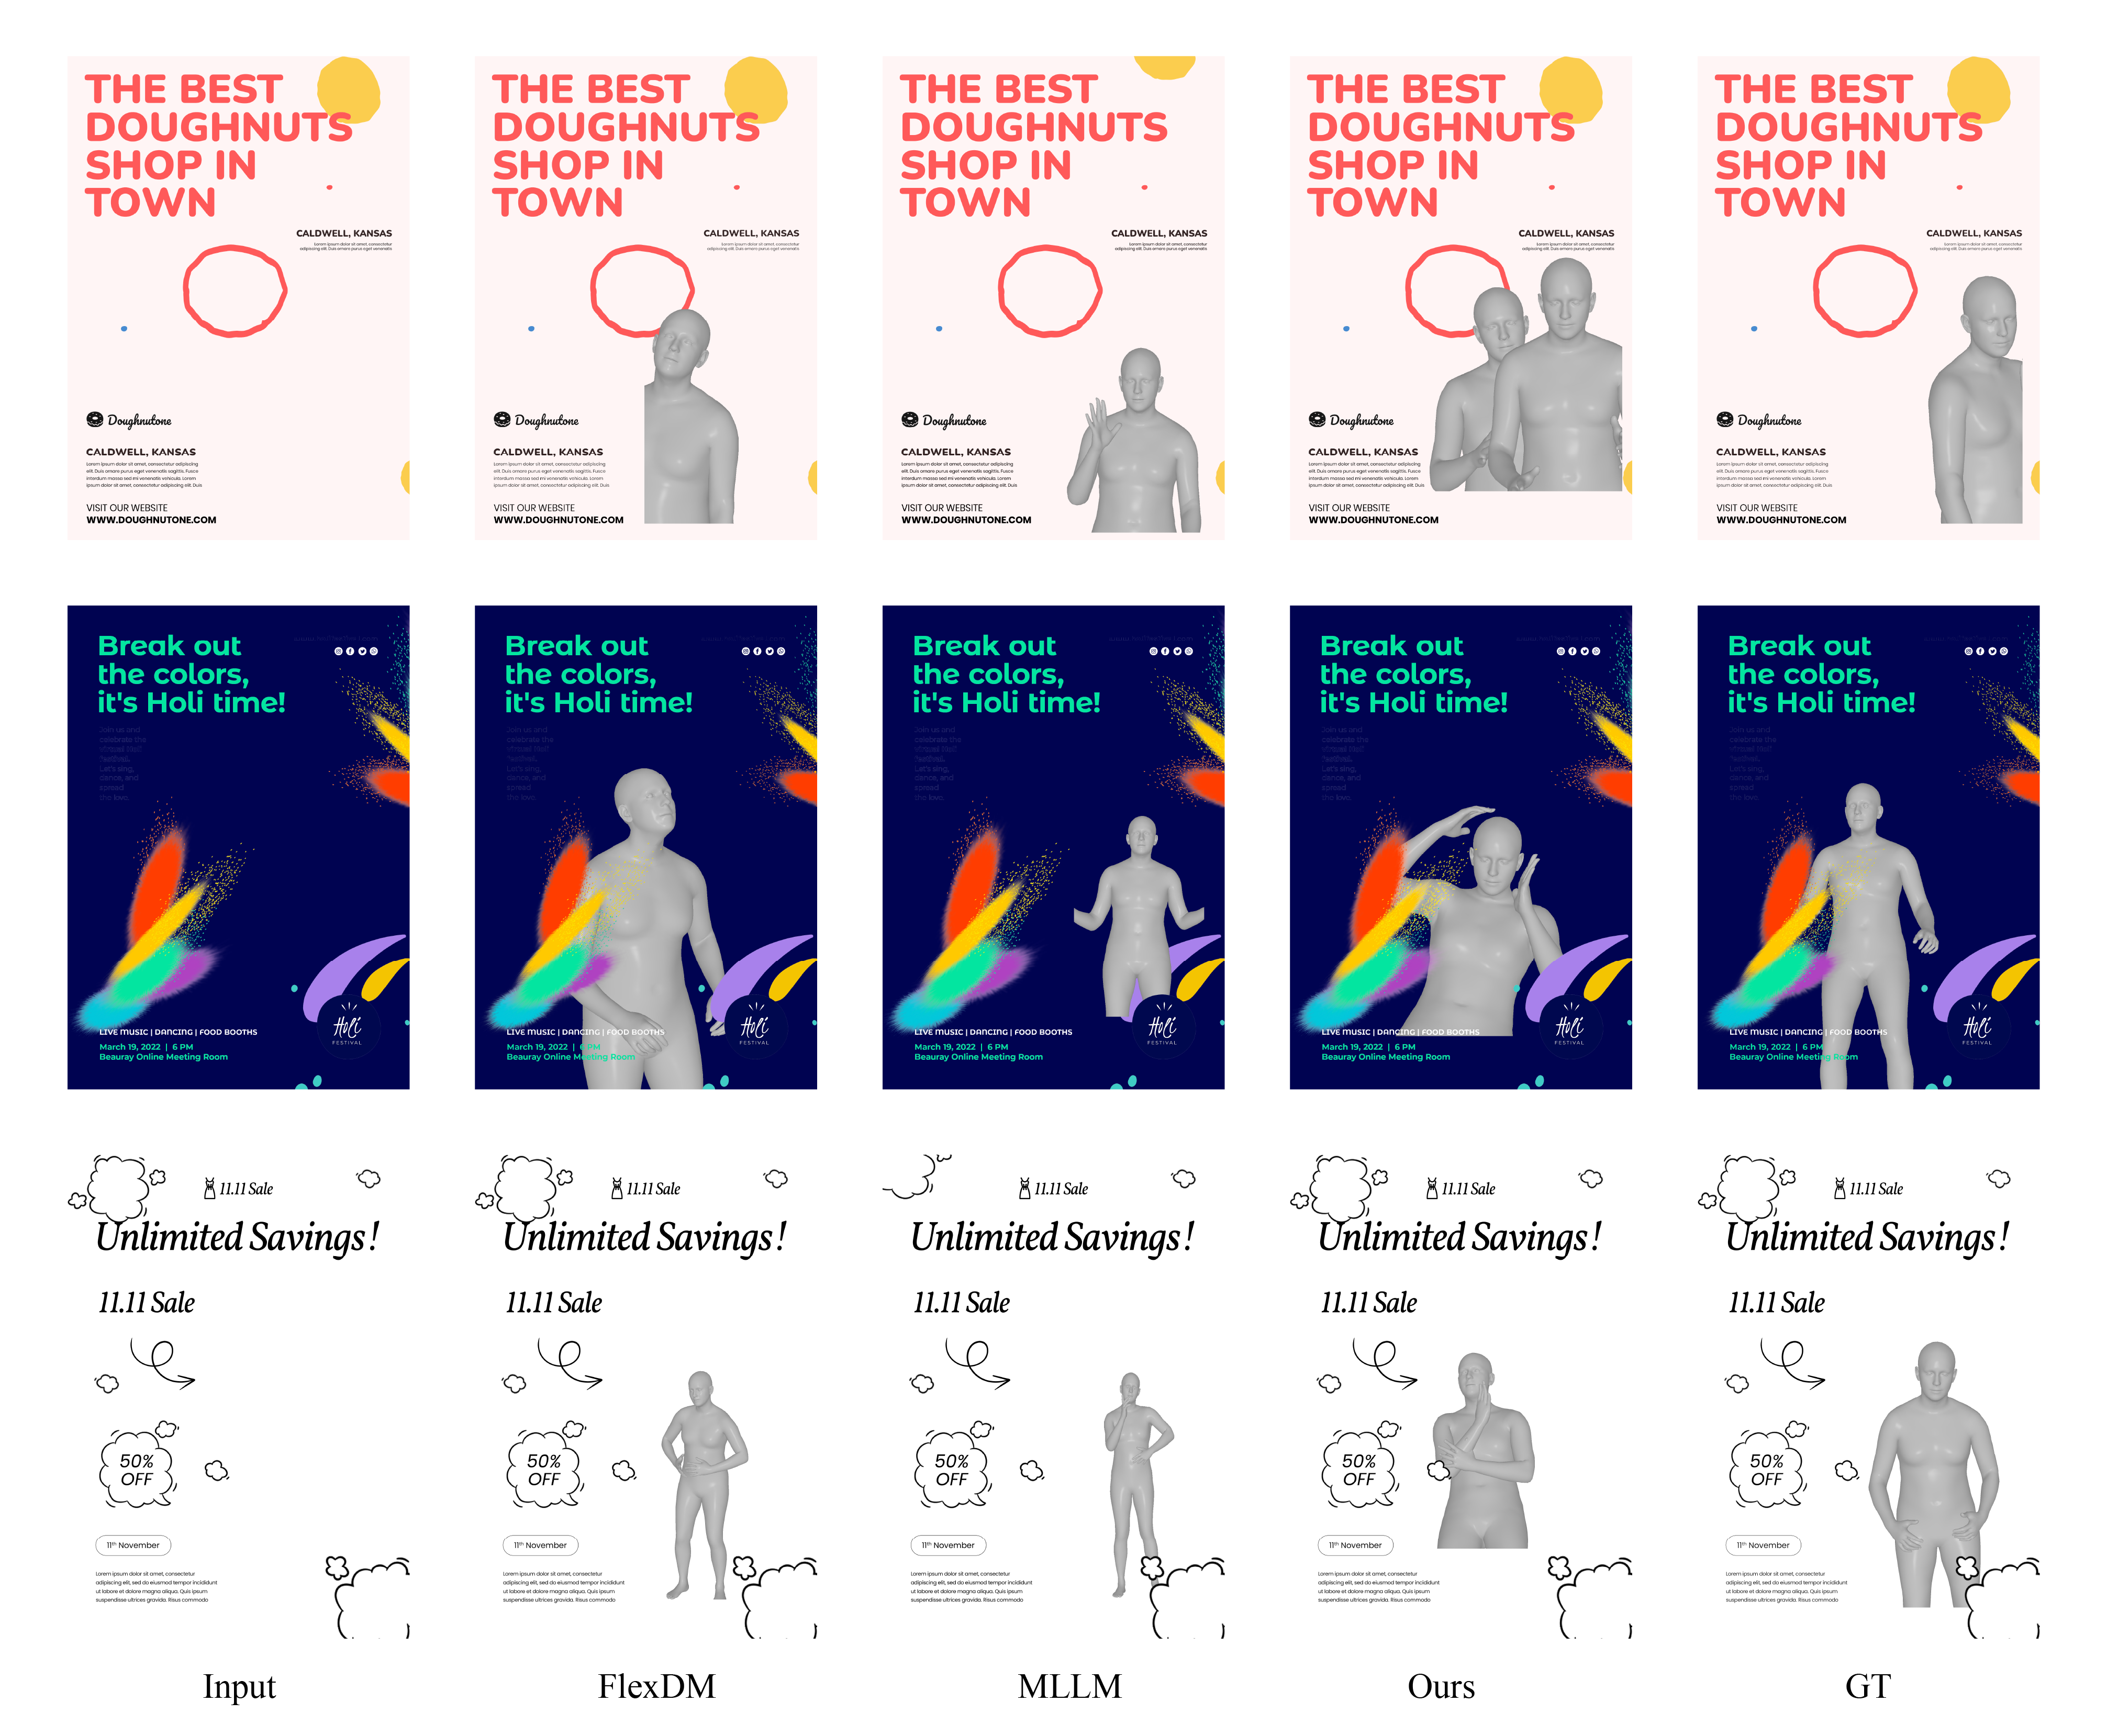
\includegraphics[width=0.85\linewidth]{figure/fig6_more_comparison.png}
\caption{Qualitative comparison of different methods.}
\label{fig:more_comparison}
\end{figure*}

\section{Additional User Study}
we conduct a user study with professional graphic designers to evaluate the results from three methods: FlexDM, MLLM, our method. For each method, we apply it to 100 input designs from our test set to generate complete designs where \textit{human mesh images}, instead of realistic human images, are added. The participants are presented with three generated designs by the three methods, along with the input design and ground truth design for reference, and choose the best generated design for each of the five aspects: 1) \textit{human-design alignment} (whether the added human image fits well with the design context); 2) \textit{pose-design alignment} (whether the human pose fits well with the design context); 3) \textit{framing-design alignment} (whether the framing fits well with the design context); 4) \textit{layout-design alignment} (whether the human image layout fits well with the design context); 5) \textit{aesthetic quality} (whether the design looks visually aesthetic). The results are shown in Table~\ref{tab:user_study_supp}. Our method is strongly preferred over the other methods across all the aspects.

\begin{table}[H]
\centering
\caption{User study results. For each aspect, the percentage of the time that each method is chosen as the best is reported.}
\label{tab:user_study_supp}
\resizebox{0.8\columnwidth}{!}{%
\begin{tabular}{l|ccc}
\hline
Aspect & FlexDM & MLLM & Ours \\
\hline
Human-Design Align  & 14.3\% & 25.2\% & \textbf{60.5\%} \\
\hline
Pose-Design Align               & 13.5\% & 17.4\% & \textbf{69.1\%} \\
Framing-Design Align     & 23.3\% & 31.1\% & \textbf{45.6\%} \\
Layout-Design Align & 19.8\% & 30.9\% & \textbf{49.4\%} \\
\hline
Aesthetic Quality  & 16.2\% & 19.6\% & \textbf{64.2\%} \\
\hline
\end{tabular}%
}
\end{table}

\section{Ablation on the Training Strategy}

As shown in Table~\ref{tab:ablation_training}, our three-stage training strategy outperforms a single-stage baseline that jointly trains both generators in a single stage, suggesting its effectiveness.

\begin{table}[H]
\centering
\caption{Ablation on our training strategy. 
The best results are in bold.}
\label{tab:ablation_training}
\resizebox{\columnwidth}{!}{%
\begin{tabular}{l|ccccc}
\hline
Method & HD-Align~$\uparrow$ & D-FID~$\downarrow$
& MPJPE~$\downarrow$
& Align~$\downarrow$ & \textbf{Overlap}~$\downarrow$ \\
\hline
Single-stage       & 6.41 & 0.08 & 386.32 & \textbf{0.17} & 210.63 \\
Three-stage (Ours) & \textbf{6.52} & \textbf{0.07} & \textbf{385.12} & \textbf{0.17} & \textbf{210.48} \\
\hline
\end{tabular}%
}
\end{table}

\end{document}

